\newpage

\section{Softwarearchitektur}

\subsection{Komponentenarchitektur}
Die Software ist objektorientiert und modular aufgebaut. Die verschiedenen Teilfunktionen als auch die Harwaretreiber sind in eigene Komponenten eingebettet. Die Komponenten können über eine schmale vordefinierte Schnittstelle angesprochen werden. In der Abbildung \ref{fig:komponentenmodell} ist das Komponentenmodell abgebildet. Der Modulare Aufbau und die Schnittstellen erlauben es, eine Komponente komplett auszutauschen. Als Beispiel wurde ein \texttt{TofAlignmentChecker} durch einen \texttt{UltrasonicAlignmentChecker} ausgetauscht. Dies konnte ohne jegliche Codeänderungen in anderen Komponenten vorgenommen werden.

\begin{figure}[H]
  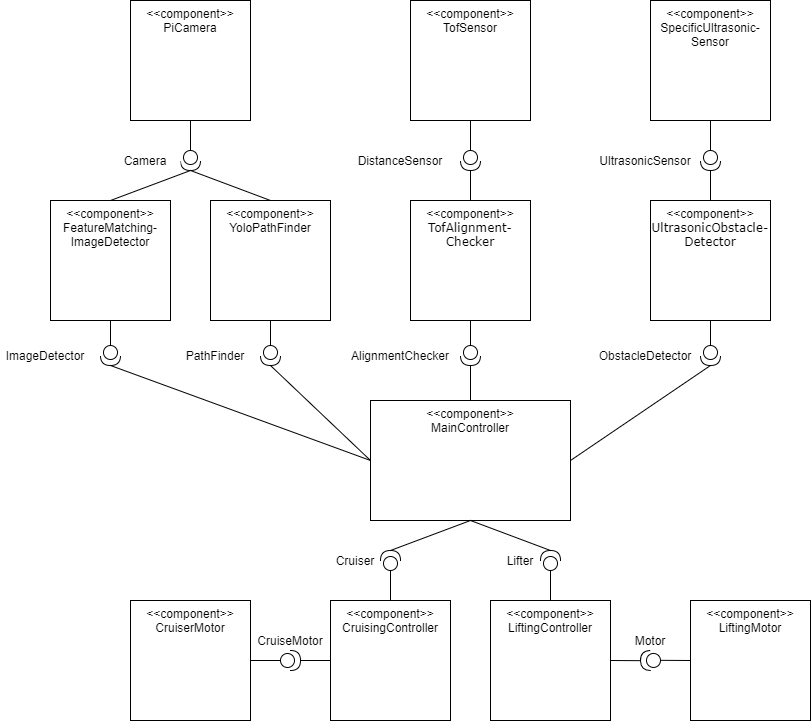
\includegraphics[width=1\textwidth]{img/softwarearchitektur/Softwarearchitektur.png}
  \centering
  \caption{Komponetenmodell}
  \label{fig:komponentenmodell}
\end{figure}

\newpage

\subsubsection{Main Controller}
Der Main Controller ist der Kern, welche die restlichen Komponenten zielbringend orchestriert. Innerhlab des Main Controllers befindet sich eine Finite State Machine:\\ \texttt{StairClimbingFrog}. Diese ist im Kapitel \ref{sec:fsm} beschrieben. 

In der Abbildung \ref{fig:uml-main} ist zusehen, dass die verschiedenen Zustände und Unterzustände mithilfe von Enumerationen realisiert werden. Dies bringt zum einen den Vorteil, dass zur Kompilierzeit ein Compilererror ausgegeben wird, wenn der Zustand nicht existiert. Wären die Zustände mithilfe von Strings realisiert, würde erst in der Laufzeit bekannt, ob die Zustände existieren oder nicht. Weiter ist der Workflow dank dem Intellisense, welches durch Enumerationen ermöglicht wird, beschleunigt.

Der \texttt{StairClimbingFrog} nimmt als Konstruktorparameter einen \texttt{ImageDetector}, \texttt{PathFinder}, \texttt{AlignmentChecker}, \texttt{ObstacleDetector}, \texttt{Cruiser} und \texttt{Lifter} entgegen. Die konkrete Implementation welche sich hinter diesen Schnittstellen befindet, kann bei der Instanzierung des \texttt{StairClimbingFrog} gewählt werden.

\begin{figure}[H]
  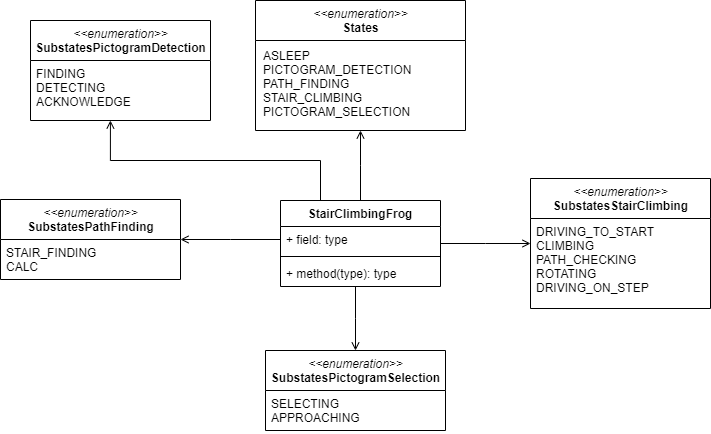
\includegraphics[width=0.95\textwidth]{img/softwarearchitektur/UML-MainController.png}
  \centering
  \caption{UML: MainController}
  \label{fig:uml-main}
\end{figure}

\newpage

\subsubsection{Lifting Controller}
Der \texttt{LiftingController} ist dazu da, den Hauptmotor anzusteuern. Er implementiert das Interface \texttt{Lifter}. Über dieses Interface kann der \texttt{LiftingController} von aussen angesprochen werden. Weiter hält er die Instanz des Motors. Das Interface \texttt{Motor} bestimmt die Methoden welche der \texttt{LiftingMotor} implementieren soll. Auch hier kann die spezifische Implementation dank dem Interface variieren, ohne dass Codeanpassungen in anderen Klassen notwendig sind. Das \texttt{I2cDevice} abstrahiert den Zugriff auf den PCA9685 Treiber \cite{pca9685-driver}, welcher über I2C angesprochen wird und PWM Signale generiert, um die Motoren zu steuern. Zur Abstrahierung wird das Python Package PCA9685-driver \footnote{https://github.com/voidpp/PCA9685-driver} verwendet.

\begin{figure}[H]
  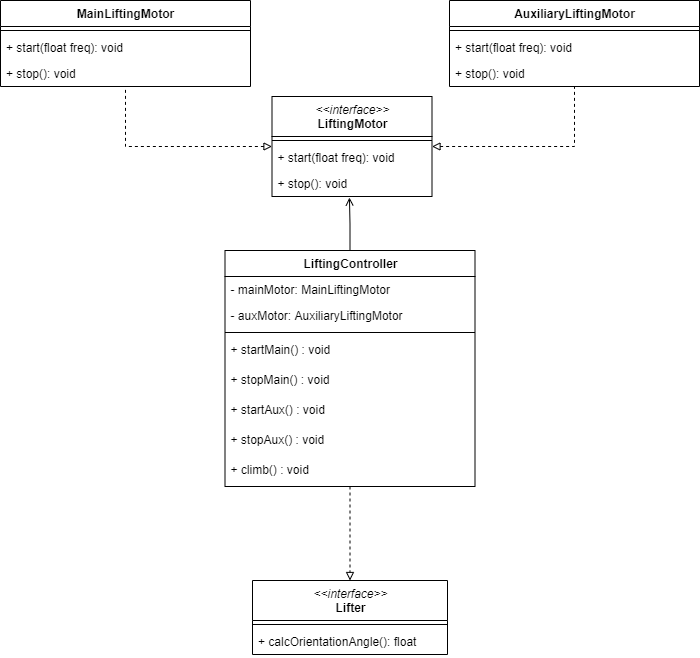
\includegraphics[width=0.95\textwidth]{img/softwarearchitektur/UML-LiftingController.png}
  \centering
  \caption{UML: LiftingController}
  \label{fig:uml-lifting-controller}
\end{figure}

\newpage

\subsubsection{Cruising Controller}
Die Komponente Cruising Controller ist grundsätzlich gleich aufgebaut wie der Lifting Controller. Über das Interface \texttt{Motor} werden die spezifischen Motorenimplementationen abstrahiert. Der \texttt{CruiseController} hat zwei Instanzen des \texttt{CruiseMotor}. Einen für das linke Rad und einen für das rechte Rad. Weiter hat er zwei Instanzen des \texttt{Encoder}. Auch hier wird wieder der PCA9685 Treiber verwendet, um die PWM Signale zu generieren, welcher durch das \texttt{I2cDevice} instanziert wird. Über die verschiedenen Methoden, welcher durch das \texttt{Cruiser} Interface vorgegeben werden, kann die Fortbewegung des Roboters gesteuert werden.

\begin{figure}[H]
  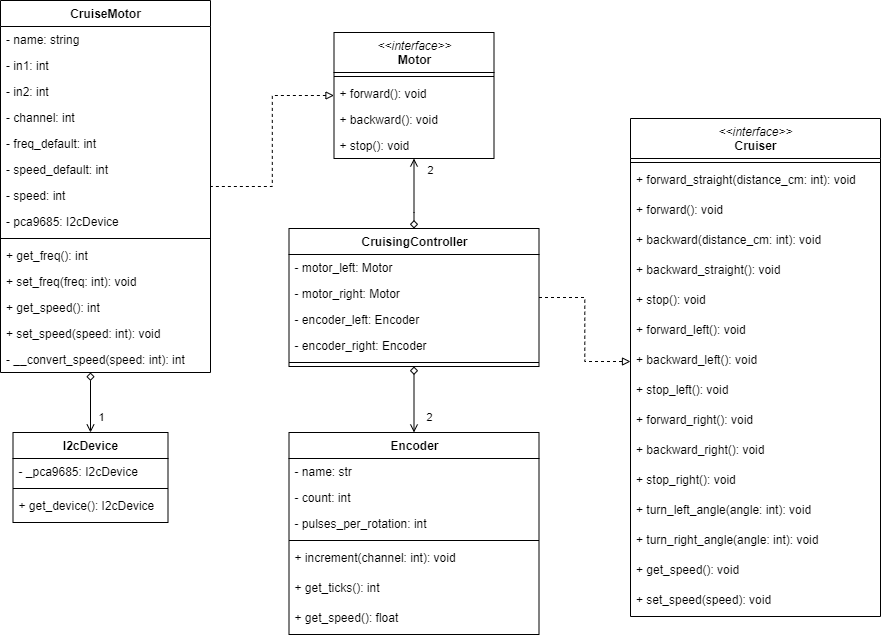
\includegraphics[width=0.95\textwidth]{img/softwarearchitektur/UML-CruisingController.png}
  \centering
  \caption{UML: CruisingController}
  \label{fig:uml-cruising-controller}
\end{figure}

\newpage

\subsubsection{Ultrasonic Alignment Checker}
\label{subsec:ultrasonic-alignment-checker}
Der \texttt{UltrasonicAlignmentChecker} hält die Instanzen von zwei \texttt{UltrasonicSensor} und liefert deren Differenz zurück. Mithilfe dieser Differenz kann sich der \texttt{StairClimbingFrog} senkrecht zur Treppe ausrichten. Auch hier werden wieder Interfaces verwendet. Welche dank Dependency Injection einen einfachen Austausch der konkreten Implementation erlauben.

In der aktuellsten Version der Software verwendet der \texttt{UltrasonicAlignmentChecker} anstelle der \texttt{UltrasonicSensor} Instanzen neu je eine Instanz des \texttt{UltrasonicLeftKernelSensor} bzw. \texttt{UltrasonicRightKernelSensor}. Die beiden Kernel-Sensoren greifen nämlich mithilfe einer kleinen Library \cite{linux-hc-sro4} welche in C programmiert wurde direkt auf den Linux-Kernel zu, um die Distanzmessung unabhängig vom Scheduler vorzunehmen. Die Erfahrung zeigte, dass Distanzmessungen mit einer High Level Programmiersprache wie Python, welche nicht wirklich real time ist, zu teilweise ungenauen Ergebnissen führte. Aus diesem Grund wurde auf die oben genannte C-Library zurückgegriffen.

\begin{figure}[H]
  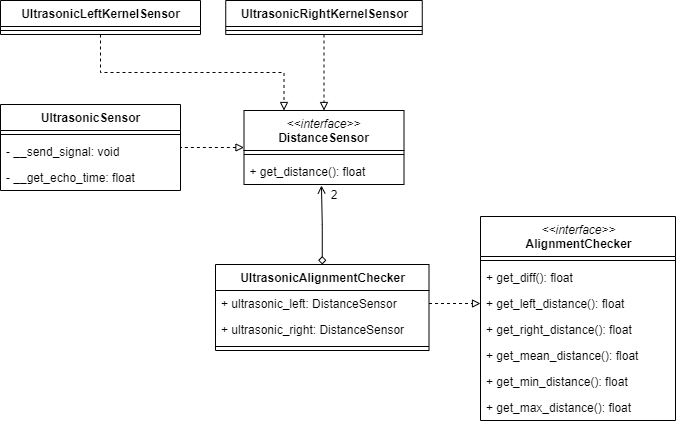
\includegraphics[width=0.95\textwidth]{img/softwarearchitektur/UML-UltrasonicAlignmentChecker.png}
  \centering
  \caption{UML: UltrasonicAlignmentChecker}
  \label{fig:uml-ultrasonic-alignment-checker}
\end{figure}

\newpage

\subsubsection{Tof Alignment Checker}
Der \texttt{TofAlignmentChecker} hält die Instanzen von zwei \texttt{TofSensor} und liefert deren Differenz zurück. Mithilfe dieser Differenz kann sich der \texttt{StairClimbingFrog} senkrecht zur Treppe ausrichten.

Der \texttt{TofAlignmentChecker} wurde gegen Ende des Projekts durch den \\ \texttt{UltrasonicAlignmentChecker} ausgetauscht und wird in der finalen Version nicht mehr verwendet. Der Grund dafür war die glänzende Oberflächenbeschaffenheit der Treppe. Das Sonnenlicht, welches von der Oberfläche reflektiert wurde, führte zu falschen Distanzergebnissen bei den TOF-Sensoren.

\begin{figure}[H]
  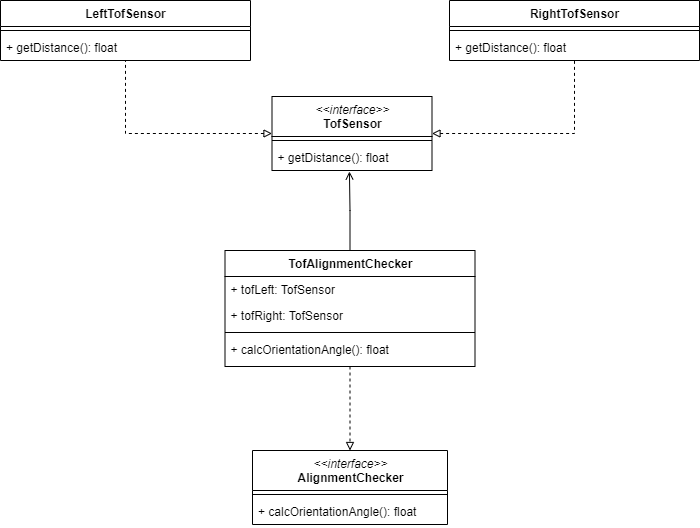
\includegraphics[width=0.95\textwidth]{img/softwarearchitektur/UML-TofAlignmentChecker.png}
  \centering
  \caption{UML: TofAlignmentChecker}
  \label{fig:uml-tof-alignment-checker}
\end{figure}

\newpage

\subsubsection{Ultrasonic Obstacle Detector}
Ähnlich aufgebaut ist der Ultrasonic Obstacle Detector. Über das Interface \texttt{ObstacleDetector} kann der \texttt{UltrasonicObstacleDetector} angesprochen werden. Dieser erkennt mithilfe seiner Instanz des \texttt{UltrasonicSensor} Hindernisse vor dem Roboter und liefert die Distanz zu diesem zurück.

Auch hier wurde auf die bereits im Kapitel \ref{subsec:ultrasonic-alignment-checker} erwähnte C-Library zurückgegriffen, um die Genauigkeit zu verbessern. Der \texttt{UltrasonicFrontKernelSensor} misst die Distanz also in einer nicht blockierenden, präzisen und auslastungsunabhängigen Weise.

\begin{figure}[H]
  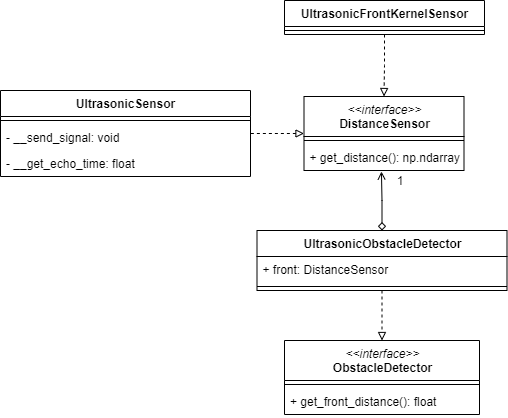
\includegraphics[width=0.95\textwidth]{img/softwarearchitektur/UML-UltrasonicObstacleDetector.png}
  \centering
  \caption{UML: UltrasonicObstacleDetector}
  \label{fig:uml-ultrasonic-obstacle-detector}
\end{figure}

\newpage

\subsubsection{Feature Matching Image Detector}
\label{sec:architecture-feature-matching}
Die Feature Matching Image Detector Komponente wird verwendet, um das Piktogramm im Startbereich zu finden und zu erkennen. Weiter ist er zuständig, um das richtige Piktogramm im Zielbereich auszuwählen. Es wäre möglich, das detektierte Piktogramm im Zielbereich in einer beliebigen Reihenfolge zu selektieren. Da die Position im Zielbereich jedoch fest vorgegeben ist, wird diese Funktionalität nicht gebraucht.
Die Klasse \texttt{Piktogramm} repräsentiert die zu detektierende Piktogramme und deren vorbestimmte Keypoints und Deskriptoren (Features). Der \texttt{SiftImageDetector} implementiert über das Interface \texttt{Camera} eine spezifische Kamera Implementation. Für die Bilder, welche die Kamera macht, werden ebenfalls die Features berechnet und mit diesen der Piktogramme abgeglichen. Der Main Controller kann über das \texttt{ImageDetecotr} Interface die entsprechenden Methoden des \texttt{SiftImageDetector} aufrufen.

\begin{figure}[H]
  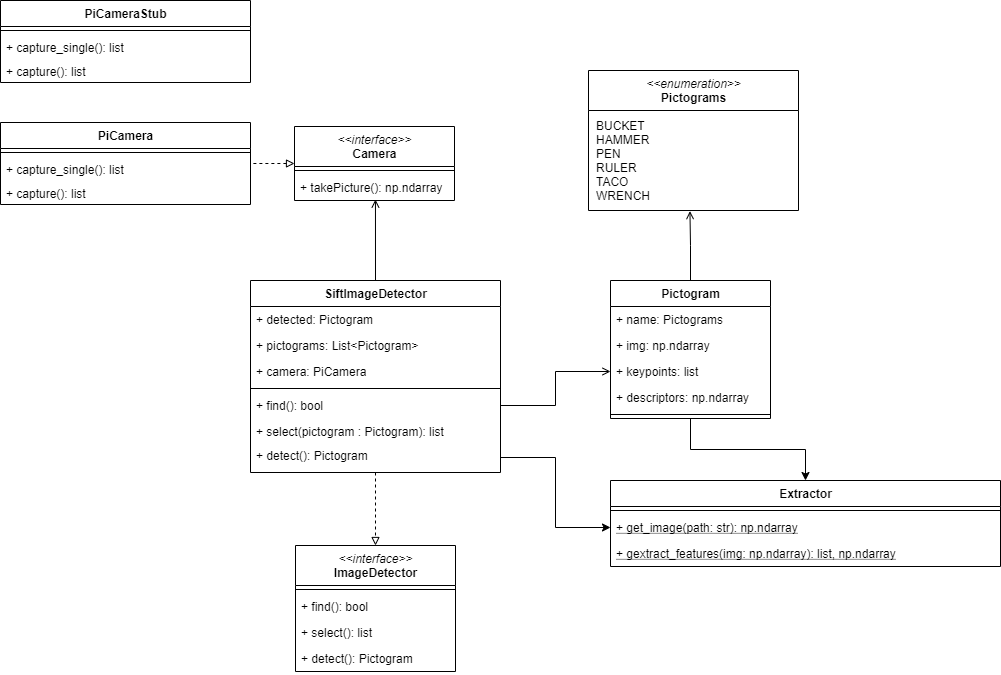
\includegraphics[width=1\textwidth]{img/softwarearchitektur/UML-FeatureMatchingImageDetector.png}
  \centering
  \caption{UML: FeatureMatchingImageDetector}
  \label{fig:uml-feature-matching-image-detector}
\end{figure}

Der \texttt{Extractor} ist eine Hilfsklasse mit statischen Methoden, welche Bilder in ein numpy array einliest, in Graustufen konvertiert, leicht verzerrt und auf eine Einheitliche Grösse skaliert. Weiter werden statische Methoden angeboten für die Merkmalextraktion und Berechnung der Deskriptoren von verschiedenen Algorithmen.

\subsubsection{Detectron2PathFinder}
Der \texttt{Detecton2PathFinder} erkennt die Stufen und Hindernisse auf der Treppe und berechnet daraus eine Matrix. Dies wird mit der \texttt{find\_path(...)} Methode der \texttt{PathFinder} Schnittstelle realisiert. Der optimale Pfad durch die Matrix wird mithilfe des \texttt{AstarFinders} berechnet.

\begin{figure}[H]
  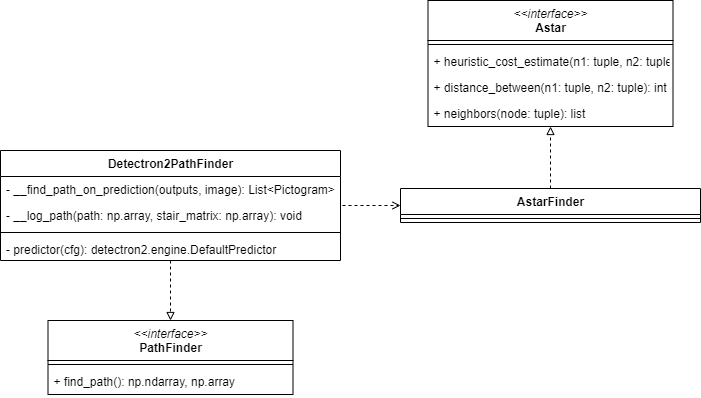
\includegraphics[width=1\textwidth]{img/softwarearchitektur/UML-PathFinder.png}
  \centering
  \caption{UML: Detectron2PathFinder}
  \label{fig:detectron2-path-finder}
\end{figure}

\newpage

\subsubsection{Camera}
Die \texttt{BashCam} war die erste Version der Kamera, welche für jedes Bild den Kamerastream öffnet, ein Bild schiesst und danach den Stream wieder schliesst. Da das öffnen des Streams jedoch etwa 6 s in anspruch nimmt, wurde die \texttt{BGCam} implementiert, welche den Stream in einem Thread kontinuierlich laufen lässt. Die \texttt{BGCam} ist ein Singleton, da lediglich ein Stream geöffnet werden darf.

\begin{figure}[H]
  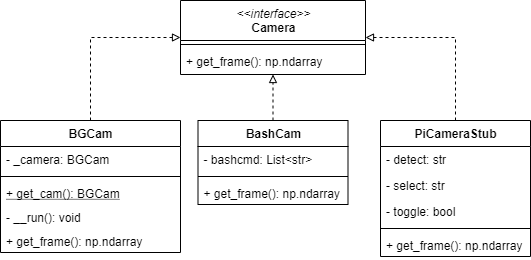
\includegraphics[width=1\textwidth]{img/softwarearchitektur/UML-Camera.png}
  \centering
  \caption{UML: Camera}
  \label{fig:uml-camera}
\end{figure}

Der \texttt{PiCameraStub} dient lediglich dem Testing. Dem \texttt{SiftImageDetector} kann mittels dependency injection die spezifsiche Kameraimplementation übergeben werden. Die Methoden des Testdoubles liefern vordefinierbare Bilder, welche beim Erzeugen des \texttt{PiCameraStubs} oder danach gesetzt werden können. Im nachfolgenden Codesnippet wird anhand eines Test-Cases die Anwendung des \texttt{PiCameraStubs} veranschaulicht.

\begin{minted}{python}
  class TestSiftImageDetectorBucket(unittest.TestCase):
    train_path = os.path.join(os.getcwd(), "image_detector", "img", "train")
    test_path = os.path.join(os.getcwd(), "image_detector", "img", "test")

    def test_detect_bucket(self):
        print("\n--- Start test detect bucket on test set ---")
        detectImage = os.path.join(self.test_path, "2021-04-17T13-28-52.jpg")
        selectImage = ""
        stub = PiCameraStub(detectImage, selectImage)
        detector = SiftImageDetector(camera = stub)
        self.assertEqual(detector.detect().name, Pictograms.BUCKET)
        
    ...
 \end{minted}
 
 \subsubsection{Acknowledger}
 Der \texttt{LedAcknowledger} ist eine simple Klasse welche für verschiedene Piktogramme verschieden oft blinkt, um diese zu quittieren. Die Blinkfrequenz beträgt 2 Hz. In der Tabelle \ref{tab:piktogrammquittierung} ist zu sehen, für welches Piktogramm wie oft geblinkt wird.
 
\begin{center}
\begin{table}[H]
\begin{tabular}{|l|r|}
\hline
\textbf {Piktogramm} & \textbf{Blinkanzahl} \\
\hline
Hammer & 1 \\
\hline
Taco & 2 \\
\hline
Ruler & 3 \\
\hline
Bucket & 4 \\
\hline
Pen & 5 \\
\hline
\end{tabular}
\caption[Piktogrammquittierung]{Piktogrammquittierung}
\label{tab:piktogrammquittierung}
\end{table}
\end{center}

In Abbildung \ref{fig:uml-acknowledger} ist zusätzlich noch der AuidoAcknowledger zu sehen. Dieser spielt vorbereitete .mp3-Dateien über kleine Audio-Boxen ab. Diese Boxen sind über einen USB-to-Aux Konverter mit dem Jetson Nano verbunden. Im Konstruktor des \texttt{AudioAcknowledger} wird mithilfe des pacmd CLI \cite{pacmd} die richtige Ausgabequelle gewählt und das Volumen dieser Ausgabequelle auf etwas mehr als 90\% gesetzt. Nachfolgend ist der entsprechende Codeausschnitt eingeblendet.

\begin{minted}{python}
  class AudioAcknowledger(Acknowledger):
    def __init__(self):
        LOG.info(f"Start initialization of {self.__class__.__name__}")
        subprocess.run(
                ["pacmd", "set-default-sink", 
                    "alsa_output.usb-C-Media_Electronics_Inc._USB_Audio_Device-00.analog-stereo"],
                stdout=subprocess.PIPE
        )
        # 0 = 0%; 65'536 = 100% Volume
        subprocess.run(
                ["pacmd", "set-sink-volume",
                    "alsa_output.usb-C-Media_Electronics_Inc._USB_Audio_Device-00.analog-stereo", "60000"],
                stdout=subprocess.PIPE
        )
 \end{minted}

\begin{figure}[H]
  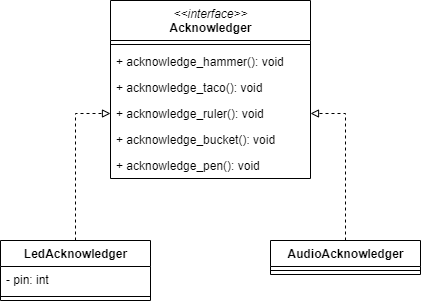
\includegraphics[width=0.6\textwidth]{img/softwarearchitektur/UML-Acknowledger.png}
  \centering
  \caption{UML: Acknowledger}
  \label{fig:uml-acknowledger}
\end{figure}

\subsection{Finite State Machine}
\label{sec:fsm}
Die Main-Komponenten regelt mithilfe einer Finite-State-Machine (FSM) den gessamten Lebenszyklus des Roboters während des Wettbewerbs. Für die Realisierung der State-Machine wird das Python Package Transitions \cite{pytransitions} verwendet. In Abbildung \ref{fig:fsm} sind die Hauptzustände modelliert. Innerhalb von jedem Hauptzustand befindet sich eine eigenständige Sub-Statemachine. Die Do-Aktivitäten innerhlab von einem Hauptzusatand werden innerhalb der Unterzustände realisiert. Für jede Do-Aktivitäten existiert ein Behavior. Ein Behavior ist eine Methode welche die benötigten Komponenten wie beispielsweise \texttt{CruisingController} und \texttt{SiftImageDetector} entgegen nimmt und mithilfe dieser die Do-Aktivität erledigt. Diese Behaviors werden automatisch bei einem Zustandsübergang durchgeführt.

\begin{figure}[H]
  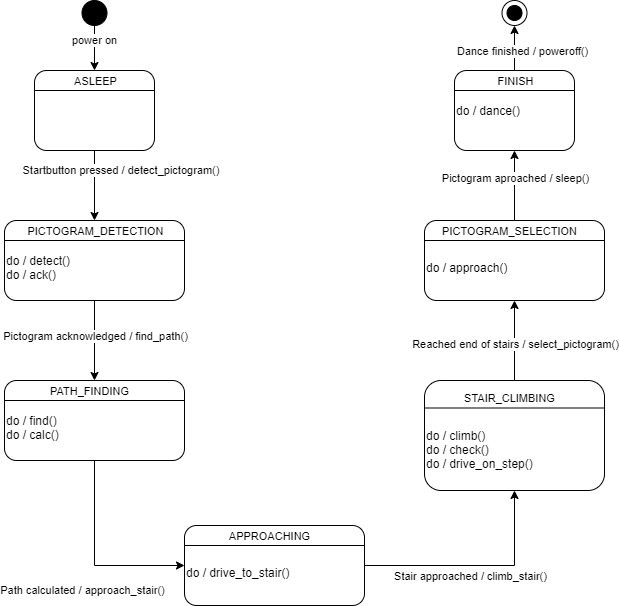
\includegraphics[width=1\textwidth]{img/softwarearchitektur/FSM-FSM.png}
  \centering
  \caption{Finite-State-Machine}
  \label{fig:fsm}
\end{figure}

\newpage

\subsubsection{Piktogramm Detektion}
In der Abbildung \ref{fig:fsm-pictogrammdetection} sind die Unterzustände der Piktogrammdetektion zu sehen. Im Unterzustand DETECTING wird das Behavior \texttt{detect\_pictogram} ausgeführt und im Unterzustand ACKNOWLEDGE das Behavior \texttt{acknowledge}.

Der Roboter wird zu Beginn so ausgerichtet, dass er auf die Treppe zeigt. Im Zustand DETECTING dreht sich der Roboter mit 40\textdegree\ im Kreis und versucht die Piktogramme zu detektieren. Da der Kamerawinkel 62.2\textdegree\ beträgt, kann der Roboter die gesamten 360\textdegree\  mit 9 Rotation absuchen. Dabei merkt er sich die Anzahl 40\textdegree \ Rotationen. Sobald das Piktogramm gefunden wurde, dreht er sich entweder in die gleiche Richtung zurück oder in die entgegengesetzte Richtung. Je nachdem ob mehr oder weniger als 3 Rotationen benötigt wurden, um das Piktogramm zu detektieren. Parallel dazu wird das Piktogramm mithilfe von blinkenden LEDs und einer Audioausgabe quittiert.

\begin{figure}[H]
  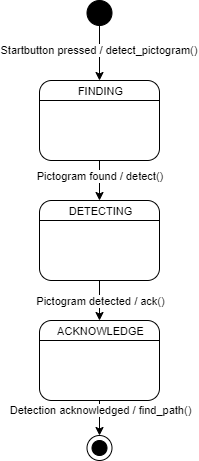
\includegraphics[width=0.40\textwidth]{img/softwarearchitektur/FSM-PICTOGRAM_DETECTION.png}
  \centering
  \caption{FSM: Piktogrammerkennung}
  \label{fig:fsm-pictogrammdetection}
\end{figure}

\newpage

\subsubsection{Pfadfindung}
In der Abbildung \ref{fig:fsm-pathfinding} sind die Unterzustände der Pfadfindung zu sehen. Im Unterzustand STAIR\_FINDING wird das Behavior \texttt{approach\_stair.py} durchgeführt. In diesem Behavior richtet sich der Roboter ca. 1.5 m mittig zur Treppe aus, damit optimale Bilder für die Pfadberechnung geschossen werden können. Danach wird das Behavior \texttt{pathfind.py} im Unterzustand CALC ausgeführt, welches ein Bild von der Treppe schiesst, mithilfe des Modells die Stufen und Ziegelsteine erkennt und den optimalen Pfad berechnet.

\begin{figure}[H]
  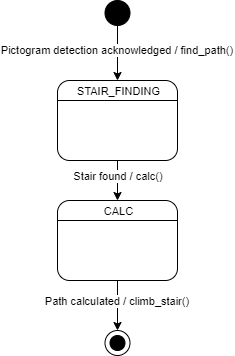
\includegraphics[width=0.40\textwidth]{img/softwarearchitektur/FSM-PATH_FINDING.png}
  \centering
  \caption{FSM: Pfadfindung}
  \label{fig:fsm-pathfinding}
\end{figure}

\newpage

\subsubsection{Treppensteigen}
\label{subsubsec:treppensteigen}
In der Abbildung \ref{fig:fsm-stair-climbing} sind die Unterzustände der Treppenerklimmung zu sehen. Im Unterzustand DRIVING\_TO\_STAIR fährt der Roboter an die optimale horizontale Position vor der Treppe um die erste Hubbewegung durch zu führen. Die horizontale Position vor der Treppe wird mit den Behaviors \texttt{calc\_pos\_infron\_stair.py} und \texttt{adjust\_pos\_infront\_stair.py} erreicht. Zu diesen Verhalten mehr im Kapitel \ref{subsec:behavior-overview}.

Im Unterzustand \texttt{CLIMBING} wird das Behavior climb\_step ausgeführt. Dieses justiert den Abstand zur Treppe auf 28 cm und startet dann die Hubbewegung. Die Hubbewegung wird so lange durchgeführt, bis sich die Ausleger wieder in der Ausgangsposition befinden. Befinden sich auf den darauf folgenden Stufen Hindernisse, kommt der Roboter in den Unterzustand \texttt{DRIVING\_ON\_STEP}. Innerhalb dieses Unterzustand wird das Behavior traverse.py ausgeführt, welches den Roboter seitlich auf der Stufe anhand des berechneten Pfades verschiebt.

\begin{figure}[H]
  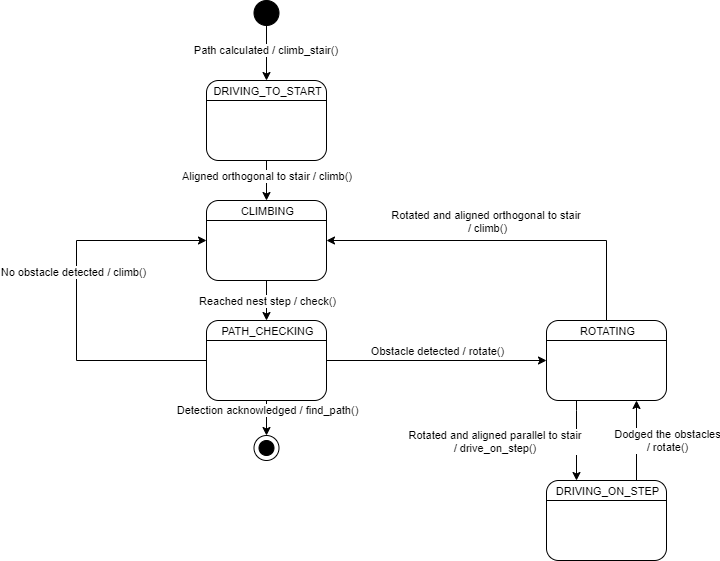
\includegraphics[width=1\textwidth]{img/softwarearchitektur/FSM-STAIR_CLIMBING.png}
  \centering
  \caption{FSM: Treppensteigen}
  \label{fig:fsm-stair-climbing}
\end{figure}

\newpage

\subsubsection{Piktogrammselektion}
In der Abbildung \ref{fig:fsm-pictogram-selection} sind die Unterzustände der Piktogramselektion zu sehen. Im Unterzustand \texttt{APPROACHING} fährt der Roboter bis zur Mitte der Zielplattform, von da aus dreht er sich 90\textdegree nach Links und verschiebt sich horizontal auf die richtige Höhe des detektierten Piktogramms. Steht der Roboter parallel zum gewünschten Piktogramm dreht er sich 90\textdegree nach rechts zurück und fährt solange geradeaus auf das Piktogramm zu, bis er 28 cm davon entfernt ist. Danach wird eine Hubbewegung eingeleitet, welche das Piktogramm ungefähr 5\textdegree auslenkt.
\begin{figure}[H]
  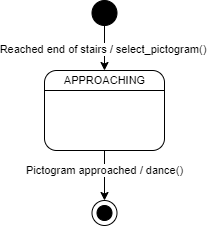
\includegraphics[width=0.40\textwidth]{img/softwarearchitektur/FSM-PICTOGRAM_SELECTION.png}
  \centering
  \caption{FSM: Piktogrammauswahl}
  \label{fig:fsm-pictogram-selection}
\end{figure}

\subsection{Übersicht Behaviors}
\label{subsec:behavior-overview}
\begin{center}
\begin{table}[H]
\begin{tabularx}{\textwidth}{|X|X|X|X|}
\hline
\textbf{Name} & \textbf{Kurzbeschreibung} & \textbf{Übergabeparameter} & \textbf{Zustand} \\
\hline
detect\_pictogram.py & Detektiert das Piktogramm im Startfeld und richtet sich wieder in die ursprüngliche Position aus. & Cruiser, ImageDetector & SubstatesPictogramDetection.DETECTING \\
\hline
acknowledge.py & Quittiert das detektierte Piktogramm. & Acknowledger, Acknowledger & SubstatesPictogramDetection.ACKNOWLEDGE \\
\hline
approach\_stair.py & Richtet sich optimal für die Pfadfindung zur Treppe aus. & AlignmentChecker, Cruiser & SubstatesPathFinding.STAIR\_FINDING \\
\hline
pathfind.py & Schiesst ein Bild von der Treppe, erkennt Stufen und Ziegelsteine und berechnet den optimalen Pfad. & PathFinder & SubstatesPathFinding.CALC \\
\hline
climb\_step.py & Erklimmt eine Stufe. & AlignmentChecker, Cruiser, Lifter & SubstatesStairClimbing.CLIMBING \\
\hline
traverse.py & Verschiebt auf einer Treppenstufe. & Cruiser, AlignmentChecker, ObstacleDetector & SubstatesStairClimbing.DRIVING\_ON\_STEP \\
\hline
approach\_pictogram.py & Fährt zum richigen Piktogramm im Zielbereich und lenkt dieses aus. & Cruiser, Lifter, ObstacleDetector & SubstatesPictogramSelection.APPROACHING \\
\hline
\end{tabularx}
\label{tab:behaviorübersicht1}
\end{table}
\end{center}

\label{subsec:behavior-overview1}
\begin{center}
\begin{table}[H]
\begin{tabularx}{\textwidth}{|X|X|X|X|}
\hline
align.py & Richtet sich senkrecht auf eine gewisse Distanz zu einem Objekt aus. Wird von den meisten anderen Behaviors verwendet. & AlignmentChecker, Cruiser, ObstacleDetector & In praktisch jedem Zustand. \\
\hline
calc\_pos\_infront\_stair.py & Berechnet die Position vor der Treppe. & AlignmentChecker, Cruiser & SubstatesPathFinding.STAIR\_FINDING, SubstatesStairClimbing.DRIVING\_TO\_START \\
\hline
adjust\_pos\_infront\_stair.py & Richtet sich anhand der berechneten Position in calc\_pos\_infront\_stair.py nach der gewünschten Position aus. & AlignmentChecker, Cruiser & SubstatesPathFinding.STAIR\_FINDING, SubstatesStairClimbing.DRIVING\_TO\_START \\
\hline
\end{tabularx}
\caption[Behaviorübersicht]{Behaviorübersicht}
\label{tab:behaviorübersicht}
\end{table}
\end{center}

\newpage

\subsubsection{calc\_pos\_infornt\_stair.py}
Da dieses Verhalten ein wenig komplexer ist, reicht die Beschreibung im Abschnitt \ref{subsubsec:treppensteigen} nicht aus wie bei den anderen Verhalten. Aus diesem Grund wird dies hier in einem separaten Kapitel noch ausführlicher beschrieben.

Wie bereits im Abschnitt \ref{subsubsec:treppensteigen} erwähnt, berechnet dieses Verhalten die Distanz vor der Treppe. Dies wird mithilfe des Abstandes zur Treppe, dem Neigungswinkel, den Ultraschallsensoren und Trigonometrie erreicht. Folgende Formel wird für den Algorithmus verwendet:

\[ y = tan(a \cdot \beta) \cdot d_t \]

$d_t$: Konstante Distanz zur ersten Stufe (Ankathete) \\
$\beta$: Neigungswinkel pro Iteration bzw. Rotation \\
$a$: Anzahl Rotationen  \\
$y$: Distanz zwischen Roboter und Eintrittspunkt Ultraschall (Gegenkathete) \\

Der Algorithmus funktioniert nun folgendermassen:
\begin{enumerate}
    \item Der Roboter richtet sich senkrecht auf den vorher definierten Abstand $d_t$ zur Treppen aus.
    \item Der Roboter dreht sich um 6\textdegree entweder nach links oder rechts (je nach dem, ob die Distanz zum linken oder rechten Treppenrand berechnet werden möchte) und inkrementiert den Rotationscounter.
    \item Nach der Rotation wird die Distanz zur Treppe gemessen.
    \begin{enumerate}
        \item Gehen die Distanzmessungen nicht an der Treppe vorbei ins Leere, wird die Gegenkathete mit obiger Formel berechnet und in einem Stack gespeichert. Danach wird zurück zu Schritt zwei gesprungen.
        \item Gehen die Distanzmessungen an der Treppe vorbei ins Leere, wird die letzte gültige berechnete Gegenkathete aus dem Stack zurückgegeben.
    \end{enumerate}
\end{enumerate}

\newpage

\subsection{Datenaustausch zwischen den Behaviors}
Zwischen den verschiedenen Behaviors müssen verschiedene Daten wie beispielsweise das detektierte Piktogramm oder die Verschiebungsdistanz auf der dritten Stufe ausgetauscht werden. Damit der Datenaustausch innerhalb der StateMachine reinbungslos funktioniert, wurde ein \texttt{DataTransferObject} eingeführt. Das \texttt{DataTransferObject} ist ein Singleton, welches alle Daten beinhaltet, welche die verschiedenen Behaviors untereinander austauschen müssen. In der Tabelle \ref{tab:datatransfer} sind alle ausgetauschten Daten kurz beschrieben.

\begin{center}
\begin{table}[H]
\begin{tabularx}{\textwidth}{|l|X|}
\hline
\textbf {Daten} & \textbf{Beschreibung} \\
\hline
detected\_pictogram & Das detektierte Piktogramm. \\
\hline
detect\_pictogram\_turn\_count & 2 Die Anzahl 40\textdegree-Drehungen welche benötigt wurden, um das Piktogramm zu finden. \\
\hline
actual\_step & Die aktuelle Stufe auf welcher sich der Roboter befindet (0 = Startbereich) \\
\hline
matrix & Die berechnete Matrix welche Stufen und Ziegelsteine abbildet. \\
\hline
path & Der berechnete Pfad durch die Matrix. \\
\hline
\end{tabularx}
\caption[Datenaustausch zwischen Behaviors]{Datenaustausch zwischen Behaviors}
\label{tab:datatransfer}
\end{table}
\end{center}
Das \texttt{DataTransferObject} bietet eine Methode \texttt{getStairOrientation()} an, welche die Verschiebungsrichtung und die Verschiebungsdistanz auf der aktuellen Stufe als Tupel zurück gibt. Auf jeder neuen Stufe wird also nachdem der Stufencounter inkrementiert wurde diese Methode aufgerufen, um zu erfahren, ob sofort die nächste Stufe erklommen werden kann oder zuerst noch eine Traversierung nötig ist.

\newpage

\subsection{Logging}
\subsubsection{Standard Logging}
Um die Software nachvollziehen zu können, wird das standard Python Logging Framework \cite{python-logging} verwendet. Hierzu werden die drei Log-Level: ERROR, DEBUG, INFO verwendet. 

\begin{center}
\begin{table}[H]
\begin{tabularx}{\textwidth}{|X|X|}
\hline
\textbf {Log-Level} & \textbf{Verwendung} \\
\hline
ERROR & Bei Fehler und Exceptions. \\
\hline
DEBUG & Für detaillierte Informationen welche nützlich beim debugging sind. Beispielsweise Inkrementimpulse der Encoder, gemessene Distanzen \\
\hline
INFO & Grundlegende Vorgänge wie z.B. Start Piktogramm Detektion, Start Stufenerklimmung \\
\hline
\end{tabularx}
\caption[Log-Level Beschreibung]{Log-Level Beschreibung}
\label{tab:log-level-description}
\end{table}
\end{center}
Hierfür werden zwei Appender verwendet, ein Log-File \texttt{debug.log} und die Konsole. Das Codesnippet für die Konfiguration des Loggers ist nachfolgend eingeblendet:

\begin{minted}{python}
import logging

logging.basicConfig(
    level=logging.INFO,
    format="%(asctime)s %(name)s [%(levelname)s] %(message)s",
    handlers=[
        logging.FileHandler("debug.log", mode='w'),
        logging.StreamHandler()
    ]
)
\end{minted}

In Abbildung \ref{fig:log-example} ist ein Auszug aus dem Log-File \texttt{debug.log} ersichtlich. Dieses zeigt die Initialisierungsphase mit dem minimalen Log-Level INFO. DEBUG-Logs werden also nicht angezeigt. Lediglich ERROR und INFO.

\begin{figure}[H]
  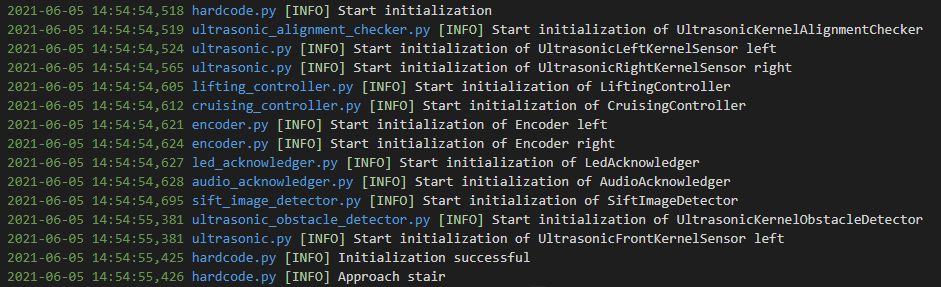
\includegraphics[width=1\textwidth]{img/softwarearchitektur/log-example.PNG}
  \centering
  \caption{debug.log der Initialisierungsphase}
  \label{fig:log-example}
\end{figure}

\subsubsection{Logging über Lautsprecher}
Neben den standardmässigen Logs in die Konsole und ins Log-File, werden die wichtigsten Ereignisse noch über den Lautsprecher ausgegeben. Hierzu wird eine natürliche Sprache verwendet, welche vom Google Übersetzer abgespielt und eingelesen wurde. Folgende Eriegnisse werden mit natürlicher Sprache ausgegeben:
\begin{enumerate}
    \item Start Initialisierung
    \item Start Piktogrammdetektion
    \item Piktogramm detektiert
    \item Start Treppenerklimmung
    \item Start der Piktogrammauswahl auf der Zielplattform
\end{enumerate}

\subsubsection{Logging an einen Webserver}
In einem weiteren Schritt wäre es möglich einen Webserver zu konfigurieren welcher die Logs in real time dem Publikum in einer übersichtlichen Benutzerschnittstelle zur Verfügung stellt. Weiter könnte die Piktogrammdetektion und der berechnete Pfad visualisiert werden. Zudem könnte der Kamerastream ausgegeben werden, damit ersichtlich ist, was der Roboter alles im Blickfeld hat.